\documentclass[12pt]{article}
\usepackage{amsmath, fullpage}
\usepackage{amssymb}
\usepackage{graphicx}
\graphicspath{ {./images/} }

\begin{document}

\title{Sincronización}
\author{Jesus H. Abundis}
%\date{\vspace{-5ex}}
\maketitle
\thispagestyle{empty}

\vspace{10pt}
Una manera de crear consistencia entre múltiples actualizaciones concurrentes de datos podría ser utilizar el tiempo como un ordenador canónico.
Si esto fuera viable podríamos simplemente hacer que todas las replicas de los datos apliquen las actualizaciones en el orden exacto en que ocurrieron.

Desafortunadamente no podemos depender en un reloj global en los sitemas distribuidos. 
Cada máquina tiene su reloj local y, 
sin medidas adicionales,
estos relojes no están sincronizados y no corren a la misma velocidad,
ocasionando una deriva en el reloj a través del tiempo.
En esencia, 
el tiempo es simplemente un caso especial de un estado global con el que no contamos en sistemas distribuidos.

\begin{figure}[h]
   \centering
   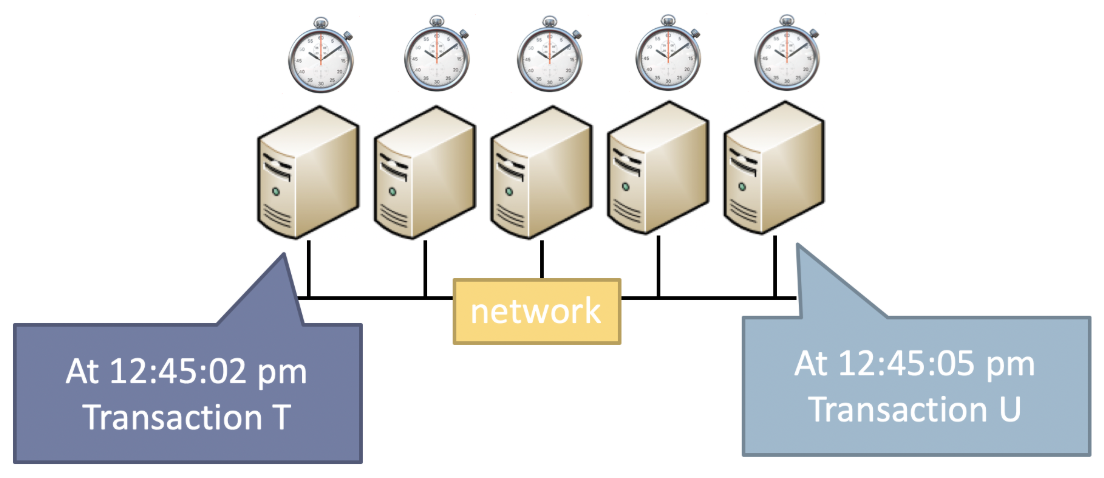
\includegraphics[scale=0.5]{red_distribuida.png}
\end{figure}

Mientras existen enfoques para sincronizar relojes en tiempo real, 
tales como NTP y Truetime, 
algunos sistemas pueden tolerar no conocer el tiempo exacto.
Por ejemplo,
un juego que emplea una simulación distribuida puede no importarle cuando ocurre cada acción exactamente.
Sólo necesita saber en que paso de la simulación se realiza cada acción.
Esto reduce el problema a determinar el orden de las acciones,
en lugar del momento exacto de cada acción.
Los relojes lógicos son una solución bien conocida para decidir el orden de las operaciones. 
Aquí discutimos dos ejemplos bien conocidos de tales relojes:
los relojes Lamport y relojes vectoriales.

Los relojes Lamport no llevan un registro del tiempo real sino que cuentan el número de eventos en una máquina. 
Enviar y recibir mensajes cuentan como eventos.
Al algoritmo no le importa qué más cuenta como evento.
Esto produce un incremento monotónico del valor en todas las máquinas.
Los relojes Lamport se construyen alrededor del concepto de una relación pasó-antes entre eventos.
Si $a$ y $b$ son eventos, 
entonces $a \to b$ significa que el evento $a$ ocurrió antes que el $b$.
Los siguientes pares de eventos tienen relaciones pasó-antes:

\begin{enumerate}
   \item Todos los eventos que ocurren en un único sistema tienen una relación pasó-antes.

   \item Los eventos que ocurren en diferentes equipos tiene una relación pasó-antes si se encuentran conectados mediante el envío y recepción de mensajes.
   Si un proceso $P1$ envía un mensaje a $P2$, 
   entonces todos los eventos en $P1$ que ocurrieron antes de la operación de envío, 
   también ocurrieron antes que todos los eventos en $P2$ en el momento en que $P2$ recibe el mensaje.
\end{enumerate}

Las equipos añaden una estampa de tiempo (su valor de reloj Lamport actual) a cada mensaje que envían. 
Un receptor compara la estampa temporal con su reloj propio.
Si la estampa temporal es menor a su valor de reloj actual no hace nada.
Por otro lado, 
cuando la estampa es mayor a su valor de reloj actual,
el receptor actualiza su reloj al valor de dicha estampa incrementado en una unidad.
Al hacer esto se garantiza que si el evento $a$ ocurrió antes que $b$,
entonces el valor del reloj lógico de $a$ es menor al de $b$.

\begin{figure}[h]
   \centering
   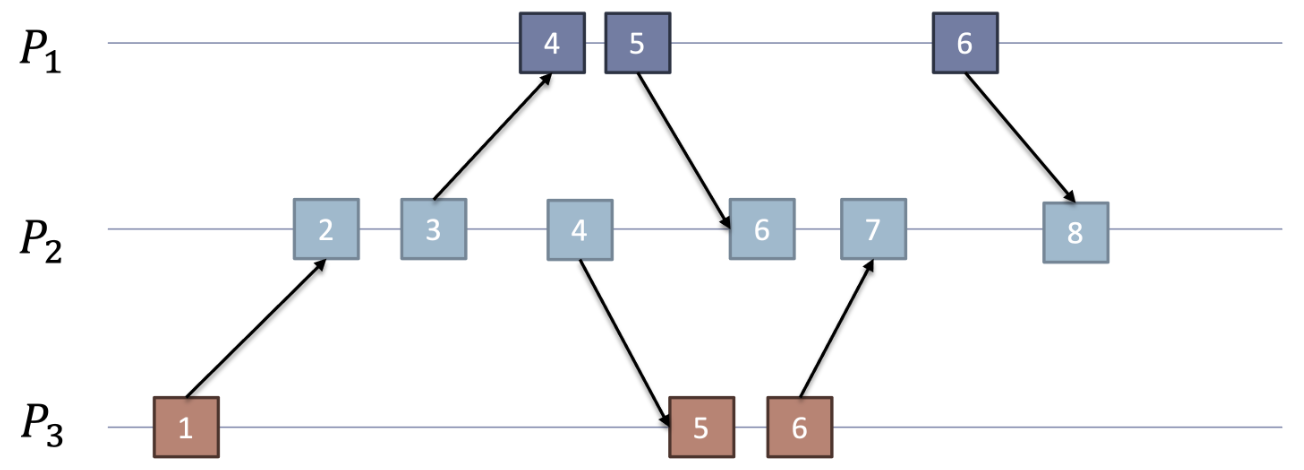
\includegraphics[scale=0.5]{Lamport_clocks.png}
\end{figure}

En esta figura se muestra un ejemplo de tres equipos utilizando relojes Lamport.
Dos eventos tienen una relación pasó-antes si existe un camino desde el primer al segundo evento ya sea moviéndose a lo largo de un mismo proceso o siguiendo un mensaje a otro proceso.
Por ejemplo, el evento con estampa 1 en el proceso $P3$ ocurrió antes que el evento con estampa 4 en $P1$.

Observa que cuando el evento enviado por el proceso $P1$ con estampa temporal 6 es recibido en $P2$,
este tiene una estampa menor a la estampa local en $P2$ (7).
El reloj Lamport se incrementa en consecuencia a 8 (el máximo entre las estampas local y del mensaje, más uno).

Los eventos que no cuentan con una relación pasó-antes se definen como \emph{concurrentes}.
En el contexto de relojes lógicos,
concurrente no significa que los eventos se ejecutan en el mismo momento.
En este caso, concurrente indica que el sistema no se ve afectado por el orden de estas operaciones;
el sistema habría llegado al mismo estado sin importar cuál evento ocurrió primero en tiempo real.
En el ejemplo superior, el mensaje enviado desde $P3$ en el momento 6 y el mensaje enviado por $P1$ en el tiempo 6 son concurrentes aún cuando no ocurrieron en el mismo instante.

Los relojes Lamport pueden utilizarse para crear un orden total en las operaciones.
Un equipo que envía un request,
agrega su valor de reloj Lamport y lo envía a todos las otras máquinas.
Los receptores colocan a los mensajes entrantes en un queue ordenado por su valor de reloj y envían un acuse de recibido al emisor y a todos los otros equipos.
De ser necesario,
las computadoras actualizan su propio valor de reloj basadas en el valor agregado en el mensaje que reciben.
Finalmente,
los equipos envían un mensaje (y lo eliminan del queue) si este se encuentra al principio del queue y si se ha notificado su recepción por parte de los otros equipos.
Una desventaja de este algoritmo es su ineficiencia;
Cada operación requiere $n^2$ mensajes para $n$ computadoras.

Aunque los relojes Lamport pueden utilizarse para generar un orden total,
el comparar dos eventos con estampas de tiempo $x$ y $y$ donde $x < y$,
no puede decirnos si $x$ ocurrió antes que $y$.
Sólo podemos concluir que $y$ no ocurrió antes que $x$,
es decir,
$x$ ocurrió antes que $y$,
o bien $x$ y $y$ son concurrentes.

En contraste, los relojes vectoriales,
los cuales son una extensión de los relojes Lamport,
capturan la causalidad.
Los relojes vectoriales nos permiten determinar,
para cada par de eventos,
cuál ocurrió primero de los dos,
o bien que son concurrentes,
simplemente inspeccionando sus valores de reloj.
Para lograr esto,
las máquinas no sólo almacenan su propio reloj Lamport
sino también el de todas las otras,
generando de esta manera un vector de relojes.

Las máquinas actualizan su propio reloj Lamport utilizando las mismas reglas utilizadas para un reloj Lamport tradicional.
Las otras entradas del vector,
es decir,
las entradas que corresponden a las otras máquinas,
se actualizan cuando se reciben los relojes vectoriales de estas.
Cada máquina agrega a cada mensaje una copia de su reloj vectorial.
Cuando los equipos reciben un mensaje,
estas actualizan su reloj vectorial incrementando su contador propio por una unidad y,
posteriormente,
actualizando las demás entradas del vector tomando el máximo entre pares de valor correspondientes.
A continuación se muestra un ejemplo de máquinas empleando relojes vectoriales:

\begin{figure}[h]
   \centering
   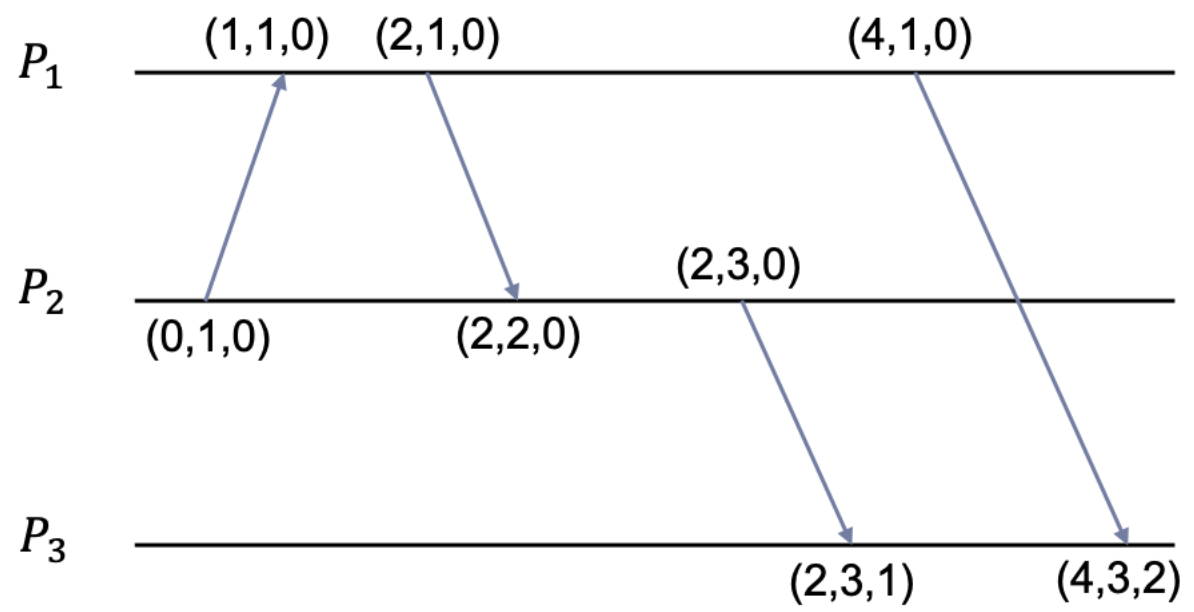
\includegraphics[scale=0.5]{vector_clocks.png}
\end{figure}

Conocer la causalidad de cada par de eventos es trivial ahora;
para un par de eventos,
$a$ y $b$,
$a$ ocurrió antes que $b$ si el vector de estampas de tiempo para $a$ es estrictamente menor que el de $b$ elemento a elemento.
Si la estampa de un evento,
no es estrictamente más grande que la estampa correspondiente al otro,
los eventos son concurrentes.
Observando la figura,
vemos que el evento con estampa (2, 1, 0) en $P1$
ocurrió antes que el evento con estampa (2, 3, 1) en $P3$,
debido a que $2 \leqslant 2$,
$1 < 3$
y
$0 < 1$.
Por otro lado,
un evento con estampa (2, 3, 0) en $P_2$,
es concurrente con un evento con estampa (3, 1, 0) en $P_1$ debido a que
$(3, 1, 0) \nleqslant (2, 3, 0)$
y
$(2, 3, 0) \nleqslant (3, 1, 0)$.

\end{document}
